% =============================================================================
\section*{Compétences}
\addcontentsline{toc}{section}{Compétences}
% =============================================================================

\begin{table}[H]
\centering
\small
\begin{tabular}{@{}p{10cm}cccc@{}}
\toprule
\textbf{Compétences} & \rotatebox{90}{\textbf{Difficile}} & \rotatebox{90}{\textbf{Familier}} & \rotatebox{90}{\textbf{Minimum}} & \rotatebox{90}{\textbf{Maîtrise}} \\
\midrule
Fournir une réponse complète à chaque question & $\square$ & $\square$ & $\square$ & $\square$ \\
Mettre les unités dans chaque nouvelle équation & $\square$ & $\square$ & $\square$ & $\square$ \\
Connaître les unités de base du SI utilisées dans Physique 1 & $\square$ & $\square$ & $\square$ & $\square$ \\
Convertir des valeurs ayant des unités simples & $\square$ & $\square$ & $\square$ & $\square$ \\
Convertir des valeurs ayant des unités composées (km/h, cm$^3$, RPM...) & $\square$ & $\square$ & $\square$ & $\square$ \\
Utiliser une équation pour déterminer les unités de base & $\square$ & $\square$ & $\square$ & $\square$ \\
S'assurer de l'homogénéité d'une équation & $\square$ & $\square$ & $\square$ & $\square$ \\
Déterminer le nombre de chiffres significatifs d'une valeur & $\square$ & $\square$ & $\square$ & $\square$ \\
Déterminer le nombre de chiffres significatifs d'une réponse & $\square$ & $\square$ & $\square$ & $\square$ \\
Utiliser sin, cos, tan et Pythagore dans un triangle rectangle & $\square$ & $\square$ & $\square$ & $\square$ \\
Utiliser les lois des sinus et du cosinus & $\square$ & $\square$ & $\square$ & $\square$ \\
Différencier une grandeur vectorielle d'une grandeur scalaire & $\square$ & $\square$ & $\square$ & $\square$ \\
Additionner et soustraire des vecteurs & $\square$ & $\square$ & $\square$ & $\square$ \\
\midrule
\multicolumn{5}{l}{\textbf{Mathématiques} (essentielles mais non enseignées dans le cours)} \\
\midrule
Isoler une variable dans une équation & $\square$ & $\square$ & $\square$ & $\square$ \\
Priorité des opérations & $\square$ & $\square$ & $\square$ & $\square$ \\
Mise en évidence & $\square$ & $\square$ & $\square$ & $\square$ \\
Distributivité & $\square$ & $\square$ & $\square$ & $\square$ \\
Proportionnalité, règle de trois, produit croisé & $\square$ & $\square$ & $\square$ & $\square$ \\
\bottomrule
\end{tabular}
\end{table}

% =============================================================================
\section*{Exercices}
\addcontentsline{toc}{section}{Exercices}
% =============================================================================

\subsection*{Questions conceptuelles}

\begin{enumerate}
    \item Énumérez les éléments qui doivent absolument faire partie d'une réponse complète.
    
    \item Énumérez les unités de base du SI qui seront utilisées dans le cours Physique 1.
    
    \item Quelle est la seule unité de base du SI à avoir un préfixe ?
    
    \item Pourquoi utilise-t-on les valeurs absolues des composantes pour calculer l'angle de référence d'un vecteur ?
    
    \item Comment détermine-t-on dans quel quadrant se trouve un vecteur à partir de ses composantes ?
    
    \item Comment s'assure-t-on qu'une équation est homogène ?
    
    \item Comment établit-on le nombre de chiffres à conserver pour la multiplication et la division ?
    
    \item Comment établit-on le nombre de chiffres à conserver pour l'addition et la soustraction ?
    
    \item À quoi doit-on penser lorsqu'on utilise la fonction arc tangente avec sa calculatrice ?
    
    \item Pourquoi ne peut-on pas simplement additionner les modules de deux vecteurs pour obtenir le module de la résultante ?
\end{enumerate}

\subsection*{Conversions}

\begin{enumerate}[resume]
    \item Convertir $l = \SI{65}{\centi\meter}$ en m 
    \hfill \textit{Rép. : $l = \SI{0,65}{\meter}$}
    
    \item Convertir $t = \SI{1,25}{\hour}$ en min 
    \hfill \textit{Rép. : $t = \SI{75,0}{\minute}$}
    
    \item Convertir $P = \SI{165}{lb}$ en kg 
    \hfill \textit{Rép. : $P = \SI{75,0}{\kilogram}$}
    
    \item Convertir $A = \SI{24,7}{\centi\meter^2}$ en \si{\meter^2} 
    \hfill \textit{Rép. : $A = \SI{24,7e-4}{\meter^2}$}
    
    \item Convertir $V = \SI{355}{mL}$ en \si{\meter^3} 
    \hfill \textit{Rép. : $V = \SI{355e-6}{\meter^3}$}
    
    \item Convertir $t = 1{,}5$ années en secondes 
    \hfill \textit{Rép. : $t = \SI{4,7e7}{\second}$}
    
    \item Convertir $p = 550\,\frac{\text{lb}\cdot\text{pi}}{\text{s}}$ en $\frac{\text{kg}\cdot\text{m}}{\text{s}}$ 
    \hfill \textit{Rép. : $p = 76{,}0\,\frac{\text{kg}\cdot\text{m}}{\text{s}}$}
    
    \item Convertir $I = \SI{101,4}{po^4}$ en \si{\milli\meter^4} 
    \hfill \textit{Rép. : $I = \SI{42,21e6}{\milli\meter^4}$}
    
    \item Convertir $p = \SI{32,0}{psi}$ en \si{\kilo\pascal} 
    \hfill \textit{Rép. : $p = \SI{221}{\kilo\pascal}$}
    
    \item Sachant que $G = \SI{6,673e-11}{\frac{\meter^3}{\kilogram\cdot\second^2}}$, $M = \SI{5,972e21}{t}$ et que $R = \SI{6374}{\kilo\meter}$, déterminez la valeur de $g = \frac{GM}{R^2}$ en \si{\meter/\second^2}.
    \hfill \textit{Rép. : $g = \SI{9,809}{\meter/\second^2}$}
\end{enumerate}

\subsection*{Chiffres significatifs}

\begin{enumerate}[resume]
    \item Combien y a-t-il de chiffres significatifs dans les valeurs suivantes : $A = 0{,}1252$ ; $B = 7{,}120$ ; $C = \num{3,726e2}$ ; $D = 155{,}1$ ; $E = 0{,}0000230$ ; $F = 4200$ ; $G = \pi$ ; $H = \frac{1}{4}$ ?
\end{enumerate}

\textit{Pour les exercices 22 à 25, réécrivez chaque valeur avec \textbf{3 chiffres significatifs} en utilisant le \textbf{préfixe SI approprié} (pas de notation scientifique). Respectez la règle : pas plus de 2 zéros après la virgule.}

\begin{enumerate}[resume]
    \item $d = \SI{0,00004520}{\meter}$
    \hfill \textit{Rép. : $d = \SI{45,2}{\micro\meter}$}
    
    \item $m = \SI{7841000}{\gram}$
    \hfill \textit{Rép. : $m = \SI{7,84}{t}$ \normalfont{(ou \SI{7,84}{\mega\gram})}}
    
    \item $t = \SI{0,00000925}{\second}$
    \hfill \textit{Rép. : $t = \SI{9,25}{\micro\second}$}
    
    \item $P = \SI{34720000}{\watt}$
    \hfill \textit{Rép. : $P = \SI{34,7}{\mega\watt}$}
\end{enumerate}

\textit{Pour les exercices suivants, donnez la réponse avec 3 C.S. en utilisant le préfixe SI approprié ou la notation scientifique.}

\begin{enumerate}[resume]
    \item Calculer $F = ma$ avec $m = \SI{12,45}{\kilogram}$ et $a = \SI{3,7}{\meter/\second^2}$.
    \hfill \textit{Rép. : $F = \SI{46,1}{\newton}$}
    
    \item Calculer $v = \sqrt{2gh}$ avec $g = \SI{9,81}{\meter/\second^2}$ et $h = \SI{4,25}{\meter}$.
    \hfill \textit{Rép. : $v = \SI{9,13}{\meter/\second}$}
    
    \item Calculer $E = \frac{1}{2}mv^2$ avec $m = \SI{0,0025}{\kilogram}$ et $v = \SI{340}{\meter/\second}$.
    \hfill \textit{Rép. : $E = \SI{144}{\joule}$}
    
    \item Calculer $P = \frac{F}{A}$ avec $F = \SI{2500}{\newton}$ et $A = \SI{0,0012}{\meter^2}$.
    \hfill \textit{Rép. : $P = \SI{2,08}{\mega\pascal}$ ou $\SI{2,08e6}{\pascal}$}
\end{enumerate}

\subsection*{Trigonométrie}

\begin{enumerate}[resume]
    \item Pour chacun des triangles suivants, déterminez les valeurs manquantes en utilisant la méthode la plus efficace.
    
    \begin{center}
    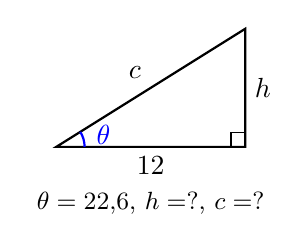
\begin{tikzpicture}[scale=0.6]
        % Triangle 1 - rectangle
        \draw[thick] (0,0) -- (4,0) -- (4,2.5) -- cycle;
        \draw (3.7,0) -- (3.7,0.3) -- (4,0.3);
        \node[below] at (2,0) {$12$};
        \node[right] at (4,1.25) {$h$};
        \node[above left] at (2,1.25) {$c$};
        \draw[thick, blue] (0.6,0) arc (0:32:0.6);
        \node[blue] at (1.0,0.25) {$\theta$};
        \node at (2,-1.2) {\small $\theta = 22{,}6°$, $h = ?$, $c = ?$};
    \end{tikzpicture}
    \hspace{0.8cm}
    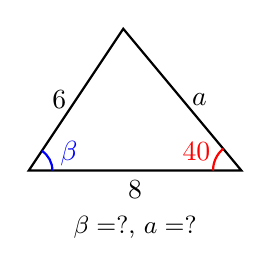
\begin{tikzpicture}[scale=0.6]
        % Triangle 2 - quelconque
        \draw[thick] (0,0) -- (4.5,0) -- (2,3) -- cycle;
        \node[below] at (2.25,0) {$8$};
        \node[right] at (3.25,1.5) {$a$};
        \node[left] at (1,1.5) {$6$};
        \draw[thick, blue] (0.5,0) arc (0:56:0.5);
        \node[blue] at (0.85,0.35) {$\beta$};
        \draw[thick, red] (3.9,0) arc (180:130:0.6);
        \node[red] at (3.55,0.4) {$40°$};
        \node at (2.25,-1.2) {\small $\beta = ?$, $a = ?$};
    \end{tikzpicture}
    \end{center}
    \hfill \textit{Rép. : $h = 5{,}00$, $c = 13{,}0$ ; $\beta = 29{,}5°$, $a = 5{,}15$}
    
    \item Un navire quitte le port et navigue \SI{15}{NM} à $45°$ par rapport à l'axe des $x$, puis \SI{20}{NM} à $150°$ par rapport à l'axe des $x$. Quelle est la distance et l'angle pour revenir directement au port ?
    
    \begin{center}
    \begin{tikzpicture}[scale=0.13]
        \draw[axe] (-12,0) -- (16,0) node[right] {\small $x$};
        \draw[axe] (0,-3) -- (0,26) node[above] {\small $y$};
        % Premier déplacement (45°)
        \draw[vecteur, line width=1.2pt] (0,0) -- (10.6,10.6);
        \node[blue, right] at (8,5) {\small 15 NM};
        \draw[thick, blue] (3,0) arc (0:45:3);
        \node[blue] at (5.5,1.5) {\small $45°$};
        % Deuxième déplacement (150°)
        \draw[vecteur rouge, line width=1.2pt] (10.6,10.6) -- (-6.7,20.6);
        \node[red, above right] at (0,17) {\small 20 NM};
        % Retour
        \draw[vecteur vert, line width=1.2pt, dashed] (-6.7,20.6) -- (0,0);
        \node[green!60!black, left] at (-5,10) {\small ?};
        \fill (0,0) circle (5pt) node[below right] {\small Port};
        \fill (-6.7,20.6) circle (5pt);
    \end{tikzpicture}
    \end{center}
    \hfill \textit{Rép. : Distance = \SI{21,7}{NM}, Angle = $288°$}
    
    \item Un câble de \SI{25}{\meter} de long est ancré au sol à \SI{18}{\meter} de la base d'un mât. Quel angle le câble fait-il avec le sol ? Quelle est la hauteur du point d'attache sur le mât ?
    
    \begin{center}
    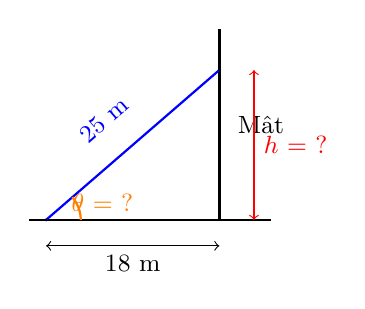
\begin{tikzpicture}[scale=0.11]
        % Sol
        \draw[thick] (-2,0) -- (26,0);
        % Mât
        \draw[very thick] (20,0) -- (20,22);
        \node[right] at (21,11) {\small Mât};
        % Câble
        \draw[thick, blue] (0,0) -- (20,17.3);
        \node[blue, above, rotate=41] at (8,10) {\small 25 m};
        % Distance au sol
        \draw[<->] (0,-3) -- (20,-3);
        \node[below] at (10,-3) {\small 18 m};
        % Hauteur
        \draw[<->, red] (24,0) -- (24,17.3);
        \node[right, red] at (24,8.7) {\small $h$ = ?};
        % Angle
        \draw[thick, orange] (4,0) arc (0:41:4);
        \node[orange] at (6.5,2) {\small $\theta$ = ?};
        % Points
        \fill (0,0) circle (5pt);
        \fill (20,17.3) circle (5pt);
    \end{tikzpicture}
    \end{center}
    \hfill \textit{Rép. : $\theta = 43{,}9°$, $h = \SI{17,3}{\meter}$}
\end{enumerate}

\subsection*{Vecteurs}

\begin{enumerate}[resume]
    \item Pour chacune des grandeurs suivantes, indiquez s'il s'agit d'un scalaire ou d'un vecteur : la vitesse, la température, la pression, le déplacement, le volume, la vitesse du vent, l'accélération, la force, l'énergie.
    
    \item Dans la méthode par composantes, que représentent les résultantes $R_x$ et $R_y$ ?
\end{enumerate}

\subsection*{Opérations vectorielles}

Les vecteurs suivants sont utilisés pour les exercices ci-dessous. 

\textbf{Pour chaque exercice :}
\begin{itemize}
    \item Dessinez les vecteurs sur un plan cartésien
    \item Donnez la réponse \textbf{en composantes} $(R_x,\, R_y)$
    \item Donnez la réponse \textbf{en module et orientation} $\|\vect{R}\| \angle \theta$
\end{itemize}

\begin{center}
\begin{tikzpicture}[scale=0.35]
    \draw[axe] (-10,0) -- (35,0) node[right] {$x$};
    \draw[axe] (0,-15) -- (0,30) node[above] {$y$};
    \draw[help lines, gray!20] (-8,-12) grid (32,27);
    % Vecteur A
    \draw[vecteur, line width=1.5pt] (0,0) -- (15,25);
    \node[blue] at (7,15) {$\vect{A}$};
    % Vecteur B
    \draw[vecteur rouge, line width=1.5pt] (0,0) -- (20,-10);
    \node[red] at (12,-8) {$\vect{B}$};
    % Vecteur C
    \draw[vecteur vert, line width=1.5pt] (0,0) -- (-8,12);
    \node[green!60!black] at (-6,8) {$\vect{C}$};
    % Vecteur D
    \draw[vecteur orange, line width=1.5pt] (0,0) -- (30,5);
    \node[orange] at (18,5) {$\vect{D}$};
\end{tikzpicture}
\end{center}

\[
    \vect{A} = 29{,}2 \angle 59{,}0° \qquad \vect{B} = 22{,}4 \angle -26{,}6° \qquad \vect{C} = 14{,}4 \angle 124° \qquad \vect{D} = 30{,}4 \angle 9{,}46°
\]

\begin{enumerate}[resume]
    \item Résoudre $\vect{R} = \vect{A} + \vect{B}$.
    \hfill \textit{Rép. : $\vect{R} = (35,\, 15) = 38{,}1 \angle 23{,}2°$}
    
    \item Résoudre $\vect{R} = \vect{B} + \vect{C}$.
    \hfill \textit{Rép. : $\vect{R} = (12,\, 2) = 12{,}2 \angle 9{,}46°$}
    
    \item Résoudre $\vect{R} = \vect{A} - \vect{B}$.
    \hfill \textit{Rép. : $\vect{R} = (-5,\, 35) = 35{,}4 \angle 98{,}1°$}
    
    \item Résoudre $\vect{R} = \vect{A} + \vect{B} + \vect{C} + \vect{D}$.
    \hfill \textit{Rép. : $\vect{R} = (57,\, 32) = 65{,}4 \angle 29{,}3°$}
\end{enumerate}

\subsection*{Solutions graphiques des opérations vectorielles}

\begin{center}
\begin{tikzpicture}[scale=0.18]
    % Exercice 31: A + B
    \begin{scope}[xshift=0cm]
        \draw[axe] (-2,0) -- (38,0) node[right] {\footnotesize $x$};
        \draw[axe] (0,-12) -- (0,28) node[above] {\footnotesize $y$};
        \draw[help lines, gray!20] (0,-10) grid (36,26);
        % A
        \draw[vecteur, line width=1.2pt] (0,0) -- (15,25) node[midway, left] {\footnotesize $\vect{A}$};
        % B à partir de A
        \draw[vecteur rouge, line width=1.2pt] (15,25) -- (35,15) node[midway, above right] {\footnotesize $\vect{B}$};
        % R
        \draw[vecteur vert, line width=1.4pt] (0,0) -- (35,15) node[midway, below] {\footnotesize $\vect{R}$};
        \node at (18,-16) {\footnotesize $\vect{R} = \vect{A} + \vect{B}$};
    \end{scope}
    
    % Exercice 32: B + C
    \begin{scope}[xshift=55cm]
        \draw[axe] (-10,0) -- (24,0) node[right] {\footnotesize $x$};
        \draw[axe] (0,-12) -- (0,16) node[above] {\footnotesize $y$};
        \draw[help lines, gray!20] (-8,-10) grid (22,14);
        % B
        \draw[vecteur rouge, line width=1.2pt] (0,0) -- (20,-10) node[midway, below] {\footnotesize $\vect{B}$};
        % C à partir de B
        \draw[vecteur vert, line width=1.2pt] (20,-10) -- (12,2) node[midway, right] {\footnotesize $\vect{C}$};
        % R
        \draw[vecteur orange, line width=1.4pt] (0,0) -- (12,2) node[midway, above] {\footnotesize $\vect{R}$};
        \node at (6,-16) {\footnotesize $\vect{R} = \vect{B} + \vect{C}$};
    \end{scope}
\end{tikzpicture}
\end{center}

\vspace{0.5cm}

\begin{center}
\begin{tikzpicture}[scale=0.18]
    % Exercice 33: A - B
    \begin{scope}[xshift=0cm]
        \draw[axe] (-8,0) -- (18,0) node[right] {\footnotesize $x$};
        \draw[axe] (0,-12) -- (0,38) node[above] {\footnotesize $y$};
        \draw[help lines, gray!20] (-6,-10) grid (16,36);
        % A
        \draw[vecteur, line width=1.2pt] (0,0) -- (15,25) node[midway, right] {\footnotesize $\vect{A}$};
        % -B à partir de A
        \draw[vecteur rouge, line width=1.2pt] (15,25) -- (-5,35) node[midway, above] {\footnotesize $-\vect{B}$};
        % R
        \draw[vecteur vert, line width=1.4pt] (0,0) -- (-5,35) node[midway, left] {\footnotesize $\vect{R}$};
        \node at (5,-16) {\footnotesize $\vect{R} = \vect{A} - \vect{B}$};
    \end{scope}
    
    % Exercice 34: A + B + C + D
    \begin{scope}[xshift=45cm]
        \draw[axe] (-5,0) -- (60,0) node[right] {\footnotesize $x$};
        \draw[axe] (0,-12) -- (0,38) node[above] {\footnotesize $y$};
        \draw[help lines, gray!20] (-3,-10) grid (58,36);
        % A
        \draw[vecteur, line width=1.2pt] (0,0) -- (15,25) node[midway, left] {\footnotesize $\vect{A}$};
        % B à partir de A
        \draw[vecteur rouge, line width=1.2pt] (15,25) -- (35,15) node[midway, above right] {\footnotesize $\vect{B}$};
        % C à partir de A+B
        \draw[vecteur vert, line width=1.2pt] (35,15) -- (27,27) node[midway, right] {\footnotesize $\vect{C}$};
        % D à partir de A+B+C
        \draw[vecteur orange, line width=1.2pt] (27,27) -- (57,32) node[midway, above] {\footnotesize $\vect{D}$};
        % R
        \draw[line width=1.6pt, purple, -{Stealth[length=3mm, width=2mm]}] (0,0) -- (57,32) node[midway, below right] {\footnotesize $\vect{R}$};
        \node at (28,-16) {\footnotesize $\vect{R} = \vect{A} + \vect{B} + \vect{C} + \vect{D}$};
    \end{scope}
\end{tikzpicture}
\end{center}
